%! TEX root = ../main.tex
% ==============================================================
% IMMUTABLE — generated automatically, do not edit this block
%
% — Provenance ───────────────────────────────────────────────────
%   script            : analysis_scratch/damping_ka_per_volt.py
%   computed_in       : analysis_scratch/damping_ka_per_volt.py (single-voltage scatter, 10V)
%   plot_type         : damping_ka
%   data_class        : DELEG
%   generated_at      : 2026-04-24T12:34:24
%   findings_doc      : memory/methodology_wind_enhances_A_in.md
%
% — Thesis context ──────────────────────────────────────────────
%   chapter           : 05
%   caption_label     : fig:ch05_damping_ka_10V
%   caption_short     : 
%
% — Filters ────────────────────────────────────────────────────
%   panel             : full
%   wind              : no + full
%   amplitude [V]     : 0.1
%   frequency [Hz]    : 1.3–1.6
%   probes            : 
%   run_category      : 
%   quality_flag      : ok
%   mooring           : 
%
% — Data provenance ────────────────────────────────────────────
%   n_runs            : 
%   in_probes_used    : 
%   out_probes_used   : 
%   probe_configs     : 
%   non_final_config_n: 
%   datasets        :
%     PROCESSED-20260326-ProbePos4_31_FPV_2-tett6roof-under9Mooring-height100-lowrange
%     PROCESSED-20260327-ProbePos4_31_FPV_2-tett6roof-under9Mooring30-height100-lowrange
%   run_paths       :
%     (omitted — aggregate over > threshold runs, see datasets)
%
% — Method / numerical parameters ─────────────────────────────
%   grouper           : 
%   collapse_panels   : 
%   fft_window_hz     : 0.1
%   extra_params      : voltage=0.10 V (tag=10V). frequency range = 1.3–1.6 Hz (thesis scope). panel condition = full. quality_flag ∈ {ok, NaN}. per-tags included: per240 + per40 (per15 excluded — window too short for H&G [50T, 60T]). datasets: PROCESSED-20260326-ProbePos4_31_FPV_2-tett6roof-under9Mooring-height100-lowrange, PROCESSED-20260327-ProbePos4_31_FPV_2-tett6roof-under9Mooring30-height100-lowrange. x-axis = IN ka (FFT) computed per run from measured IN-side wavenumber and amplitude (not derived from dispersion). y-axis = OUT/IN (FFT) from meta.json (canonical IN/OUT mean of same-distance probes; see CLAUDE.md §5). Dashed reference: ratio = 1 (no damping). Colour convention: per240 (long runs) uses thesis-wide RED = fullwind, BLUE = nowind (feedback_wind_color_convention.md). per40 (short runs) uses magenta (#D946EF) for fullwind and turquoise (#00D4BC) for nowind — chosen for hue-distance from red/blue without crossing into green/orange. Typeset in NewComputerModern10 (OTFs from TeXLive's newcomputermodern package, registered via font_manager).
%
% — Summary stats cited in caption ────────────────────────────
%   stat:n_per240_full : 10
%   stat:mean_ratio_per240_full : 0.7407
%   stat:std_ratio_per240_full : 0.0894
%   stat:ka_lo_per240_full : 0.0895
%   stat:ka_hi_per240_full : 0.1359
%   stat:n_per240_no  : 9
%   stat:mean_ratio_per240_no : 0.6264
%   stat:std_ratio_per240_no : 0.1325
%   stat:ka_lo_per240_no : 0.0506
%   stat:ka_hi_per240_no : 0.0831
%   stat:n_per40_full : 9
%   stat:mean_ratio_per40_full : 0.7289
%   stat:std_ratio_per40_full : 0.0900
%   stat:ka_lo_per40_full : 0.0903
%   stat:ka_hi_per40_full : 0.1343
%   stat:n_per40_no   : 6
%   stat:mean_ratio_per40_no : 0.5960
%   stat:std_ratio_per40_no : 0.1353
%   stat:ka_lo_per40_no : 0.0533
%   stat:ka_hi_per40_no : 0.0828
%   stat:n_freq_1p30Hz : 19
%   stat:n_freq_1p40Hz : 5
%   stat:n_freq_1p50Hz : 5
%   stat:n_freq_1p60Hz : 5
%   stat:mean_ratio_full_all : 0.7351
%   stat:n_full_all   : 19
%   stat:mean_ratio_no_all : 0.6142
%   stat:n_no_all     : 15
%
% — Subfigures available ───────────────────────────────────────
%     FIGURES/ch05_damping_ka_10V.pdf
% ── end immutable block ─────────────────────────────────────────
\begin{figure}[htbp]
  \centering
  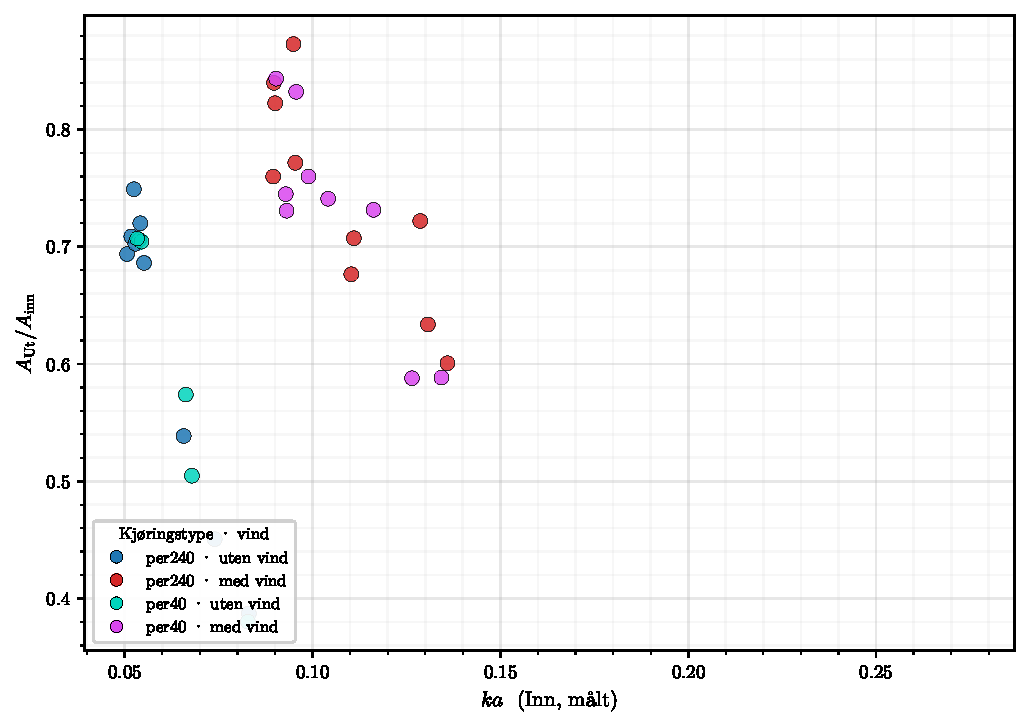
\includegraphics[width=\linewidth]{FIGURES/ch05_damping_ka_10V.pdf}
  \caption[Short caption for LOF]{
    % TODO: write caption
  }
  \label{fig:ch05_damping_ka_10V}
\end{figure}
